\documentclass[unnumsec,webpdf,contemporary,large]{oup-authoring-template}
\usepackage{hyperref}
\usepackage{xspace}
\usepackage{graphicx}
\newcommand{\zlib}{\texttt{zlib}\xspace}
\newcommand{\zran}{\texttt{zran}\xspace}
\newcommand{\ibuilder}{\texttt{index\_builder}\xspace}
\newcommand{\ireader}{\texttt{index\_reader}\xspace}
\newcommand{\gzip}{gzip\xspace}

\begin{document}

\journaltitle{CMSC701 Final Project}
\DOI{}
\copyrightyear{2023}
\pubyear{2023}
\appnotes{Final Project}

\firstpage{1}

%\subtitle{Subject Section}

\title[Compressed Checkpoint Index]{Final Project Report: Compressed Checkpoint
Index \& Parallel \gzip Reader}

\author[1]{Erik Rye}
\author[1]{Jiaxi Tang}
\author[1]{Aaron Ortwein}

%\authormark{Author Name et al.}

\address[1]{\orgdiv{Computer Science Department}, \orgname{University of
Maryland}, \orgaddress{\street{8125 Paint Branch Dr, College Park},
\postcode{20742}, \state{MD}, \country{USA}}}

%\corresp[$\ast$]{Corresponding author. \href{email:email-id.com}{email-id.com}}

%\received{Date}{0}{Year}
%\revised{Date}{0}{Year}
%\accepted{Date}{0}{Year}

\abstract{We devise and describe a tool for creating an index over a \gzip FASTQ
file. Unlike standard index-creation tools, our tool and the indices that it
creates incorporate a user-specified number of sequence reads that should be
split into each index. This allows a different tool that reads a FASTQ \gzip
file with our pre-built index over it to efficiently process the sequence reads
\emph{in parallel}, rather than needing to process the entire file serially.
This can result in a dramatic speedup for some applications, as we demonstrate
with the simple use case of reading the entire FASTQ file into memory and
writing the decompressed result back to a file.}

\keywords{FASTQ, \gzip, Compression, Parallel Processing}

% \boxedtext{
% \begin{itemize}
% \item Key boxed text here.
% \item Key boxed text here.
% \item Key boxed text here.
% \end{itemize}}

\maketitle


\section{Introduction}
Computer processors are now capable of running hundreds of threads of execution simultaneously in parallel. With severe physical limits on clock speed, future architectures will likely support more simultaneous threads rather than faster individual cores ~\cite{intropaper}. These advances provides programmers new way to speed up their programs. However, simply using more threads to exexute parts of the program does not guarantee speedup and may very well speed down than speed up. In fact, it is not uncommon for a program’s overall throughput to decrease when thread count grows large enough ~\cite{intropaper}. So, to speedup genomics software with multiple number of threads, programmers should deliberate on how they should structure the entire program and how many threads they should use so that the overhead of multithreading will not outweigh the speedup it brings.

Here we try to solve the problem of decompressing a gzip compressed FASTQ files in parallel by building indices over it. 
This startegies of building indices can scale to hundreds of threads and make it easier for our program to be part of the pipeline of other multithreading or multiprocessing genomics tools. 
\subsection{Challenge of Multithreading}
Some of the challenges multithreading will pose can be seen in Figure 1. Figure 1 shows how bad multithreading can be if handled incorrectly. We can see that if a thread needs to read from or write to a file, it needs exclusive right to the file so that the file won't be changed when it's reading it. This is usually done by using locks. Unfortunately, even though multiple threads can have read lock of the same file, operating system does not really allows them to read the file simultaneously. That means if multiple thread is trying to read a file, most of them cannot do anything and has to wait for that one thread to complete first. The same applies to writing to a file as well. Therefore, it's important to structure the program and choose parameters wisely so that the time spent waiting for each thread is minimum. 
\begin{figure}[H]
    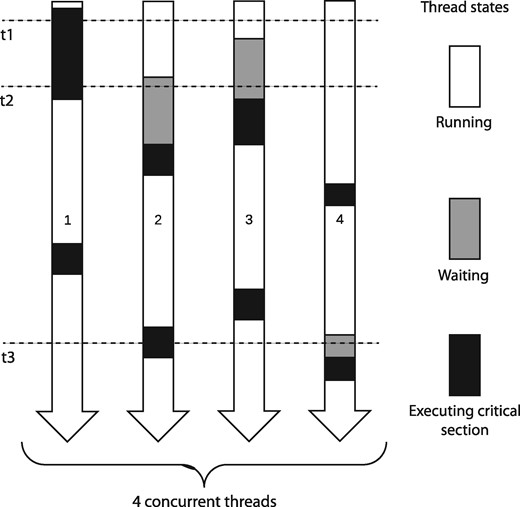
\includegraphics[width=\linewidth]{figs/multithread.jpeg}
    \label{fig:multithread}
    \caption{This figure shows 4 threads running simultaneously . Time progress from top to bottom. Gray area represents time spent waiting instead of operating. Black area represents threads doing operations that require exclusive rights to certain resources. ~\cite{intropaper}}
\end{figure}

\section{Related Work}

Kerbiriou and Chikhi examined parallel decompression of FASTQ \gzip files to
speed up genomic algorithms that require FASTQ
input~\cite{kerbiriou2019parallel}. Rather than building an index over the FASTQ file and storing the contexts needed for deflate, they decompress the gzip compressed FASTQ file by a two pass algorithm as shown by Figure 2. 
\begin{figure}[H]
    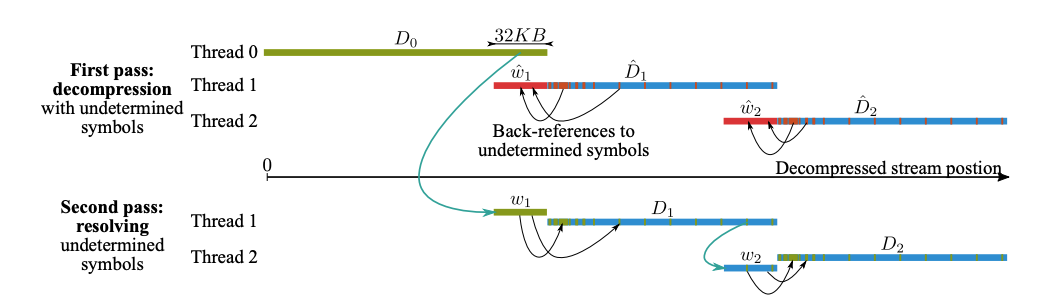
\includegraphics[scale=0.5]{figs/twopass.png}
    \label{fig:multithread}
    \caption{First pass decompress the file while leaving unresolvable back pointers untouched. The second pass will use context decompressed in the previous stream to resolve back pointers. ~\cite{kerbiriou2019parallel}}
\end{figure}
The first pass of the algorithm will divide the gzip compressed FASTQ file into multiple chunks and each thread is responsible for deflating one chunk. Since there's no context, only the thread that deflate the first chunk of the file could deflate successfully since the first chunk since every back pointer in the first chunk has to point to string within the first chunk. Because all other chunks will have back pointers that point to earlier chunk which they have access to, threads handling those chunks will mark those pointers as unresolved and deflate as much of the chunk as it can. Since the distance back pointers can point back across is 32K, the number of unresolved back pointers in each chunk is limited to 32K.
The second pass of the algorithm will then pass the last 32K bits of the deflated chunks to the threads handling later chunks so that they can resolve the unresolved back pointers. 

\texttt{zlib}~\cite{zlib} is a C library written by Mark Adler and others that
is able to create and read \gzip files. This library will be important for our
project as it exposes the underlying mechanics for inflating \gzip files.

\texttt{pyfastx}~\cite{pyfastx} is a Python C extension that enables random
reads from FASTA and FASTQ. The functionality that it exposes is similar to our
overall goal and will be a useful source of information and point of comparison.

\texttt{indexed\_gzip}~\cite{indexedgzip} is a project by Paul McCarthy to
create an index over compressed NIFTI image files, which use \gzip compression by
default. This will be another useful point of comparison in a tool that needs to
accomplish a similar task as us.

\texttt{libdeflate}~\cite{libdeflate} is a state-of-art highly optimized single-threaded open-source library used to compress and decompress files in DEFLATE/gzip/zlib format. This will serve as a great benchmark for our program.

\begin{table*}[ht]
    \centering
    \caption{Four sources of FASTQ data were used in our study. The FASTQ files
    were \gzip compressed for our index-building and parallel reading
    experiments.}
\begin{tabular}{r|l|r|r}
\multicolumn{1}{c}{\textbf{\begin{tabular}[c]{@{}c@{}}Sequence Read\\
Identifier\end{tabular}}} & \multicolumn{1}{c}{\textbf{Source}} &
    \multicolumn{1}{c}{\textbf{Sequence Reads}} & \multicolumn{1}{c}{\textbf{\begin{tabular}[c]{@{}c@{}}FASTQ GZ \\ Size (MB)\end{tabular}}} \\
\hline\\
SRR3295681 (Small)& Salmonella enterica & 959,879 & 205\\
SRR2121685 (Medium) & Mus musculus & 27,928,438 & 2,078\\
SRR925811  (Large) & Homo sapiens & 53,265,409 & 3,349 \\
SRR925816 (XL) & Homo sapiens & 71,504,007 & 5,046
\end{tabular}
    \label{tab:source}
\end{table*}

\section{Methodology}

The software tools we developed for our project consist of an \emph{index
building} component, which creates the sequence-aware \gzip index, and an
\emph{index reading} component, which we use to validate the utility of the
index building component by using the indices to read a compressed gzip file in
parallel and write it out to a file, which we then compare against the
uncompressed original FASTQ to verify our program's correctness. We first detail
the thought process and inspriation behind our approach in
Subsection~\ref{sec:zran}, document the design of our index builder in
Subsection~\ref{sec:ibuilder}, and discuss the design of the index reader and validation
tool in Subsection~\ref{sec:ireader}.

\subsection{3.1 \zran}
\label{sec:zran}

The starting point for our index creation utility is a tool called
\zran~\cite{zran}. \zran
is a single-file demonstration of how to build an index over a \gzip file
written by Mark Adler, co-creator and maintainer of \zlib. It is included with
\zlib. \zran is designed to allow for random access within a \gzip file. \zran
accomplishes this in two steps. 

First, \zran completes a full read through the \gzip file. At each \gzip block boundary, which is defined as a literal with value 256 in DEFLATE, \zran will add an access point if \zran has consumed more than SPAN number of bytes, specified by the user, and such block is not the last block. 

Then, given an offset to the uncompressed file, \zran will find an access point right before the offset and skip to the DEFLATE block that offset is in while deflating the skipped block to maintain the context needed for deflate. After the block offset is in is fetched and context for it is built, \zran will read in desired number of uncompressed bytes, decompressed them, and return the result to the user. 

\subsection{3.2 \ibuilder}
We built our \ibuilder tool around the idea of access point in \zran. By the purpose of this program, each index cannot end in the middle of a read because that will defeat the purpose of making this program part of the pipeline of other multithreading or multiprocessing genomics tools. But, because \zran was not designed for FASTQ file or genomics files in general, we have to modified \zran to add more information to our index. Therefore, we need to restrict the program to only create index when both the block and the read end. 

This, however, creates a new set of problems. The start of each DEFLATE block contains information needed to decompress the block. If the index is not on block boundary, deflate algorithm will fail to execute unless we store the Huffman code tree at the start of each block alongside the index. We decided against this approach and chose to store the index of start of the corresponding block for each index and how many uncompressed bytes we need to skip instead. 

The reason for this is simple. If the index is at the middle of a block, we have to tell deflate algorithm how many bits in the byte index points it should skip. In other words, we need to know the valid starting point in the byte which standard \zlib~\cite{libdeflate} will not provide. That means we have to write our own deflate algorithm, which is impossible due to time constraints and limitation of our knowledge about implementation of the deflate algorithm. 

The downside of this approach is quite limited considering two facts at hand. First, we won't create an index until both the block and the read at the end of the block end, which means in the worst case scenario, we only have one-read-length amount of bytes of overhead per index. Second, each read is short in FASTQ. If we can control the number of index points, we can make the overhead of our approach negligible.  
\label{sec:ibuilder}

\subsection{3.3 \ireader}
\label{sec:ireader}

\subsection{Data Sources}

We used four reference FASTQ sequence reads from the Sequence Read
Archive~\cite{SRA} for our testing and analysis. Table~\ref{tab:source} is a
tabular depiction of the data sets that we used for this project. We chose these
files because they represented a wide range of numbers of sequence reads, which
translates into a wide range of \gzip file sizes for our tool to contend with.
Indeed, the largest FASTQ \gzip file we consider is approximately 25 times as
large as the shortest.

\subsection{Index Creation Tool \& Methodology}

We implemented our solution in C in order to take advantage of the library
\zlib~\cite{zlib}. \zlib is a C library written and maintained by Jean-loup
Gailly and Mark Adler since 1995. 

\subsection{Parallel Reading}


\begin{figure}
    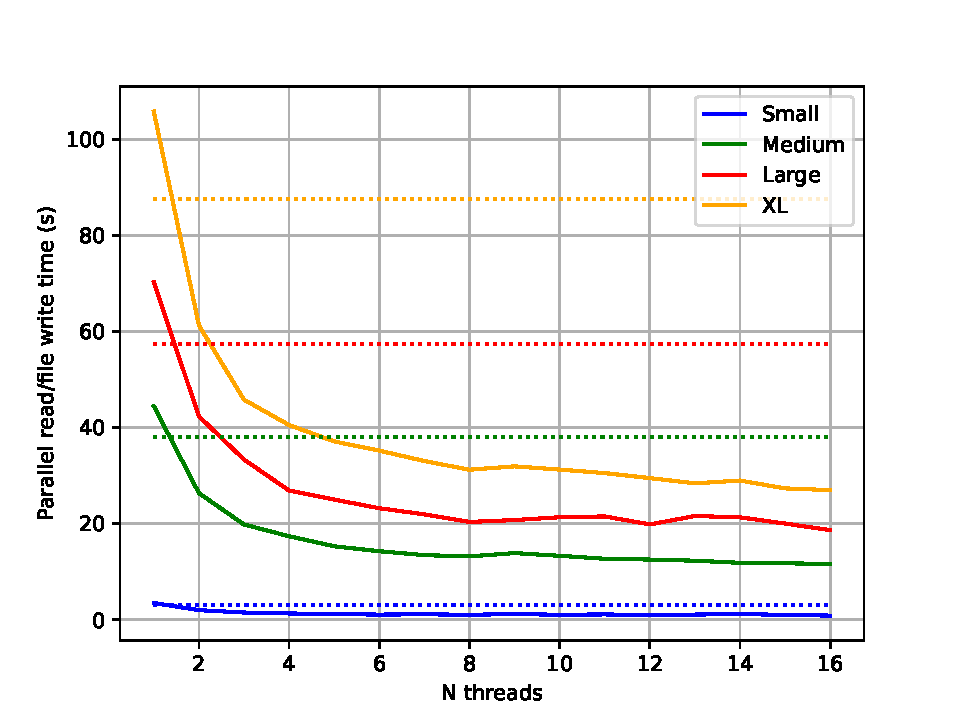
\includegraphics[width=\linewidth]{figs/cores.pdf}
    \label{fig:cores}
    \caption{Time to read differently-sized FASTQ \gzip files using a pre-built
    index file and different numbers of threads. Time compasses total program
    execution, including reading the index files, parallel reading the \gzip
    file with $N$ threads, and writing the reconstituted file to disk. Time for
    \texttt{zcat} to read the file and write it to disk is shown for comparison
    using a dotted line (\texttt{zcat} execution is single threaded). See
    Table~\ref{tab:source} for descriptions of small, medium, large, and XL.}
\end{figure}


\section{Results}

\section{Conclusion and Future Work}

Our work is located here:
\url{https://github.com/Josh-Tang112/CMSC701_Final_Project}

\bibliographystyle{plain}
\bibliography{refs.bib}


\end{document}
